%%% Template for AUTHOR's DRAFT paper in FCAA, WITHOUT Journal's head  %%%%%%%%%%%%%%%%%%%%%%%%%%%%%%%%%
%%% by V. Kiryakova, updated Nov. 1, 2014
%%% uses "fcaa.cls", or "fcaa-var.cls" as modifications of "amsart.cls" for the FCAA format,
%%% and auxiliary file "fcaa_style.tex" fixing page margins, fontsize, defs for theorems, proofs etc.
%%% Put the files "fcaa.cls", "fcaa-var.cls" and "fcaa_style.tex" in same directory you prepare the paper

  %\documentclass[twoside,reqno,11pt]{fcaa}  %%% or in case of problems, use as below: %
  \documentclass[twoside,reqno,11pt]{fcaa-var} %

 \input fcaa_style

%%%%%%%%%%%%%%%%%%%%
 \usepackage{hyperref} % Editor will use to create hyperlinks %
 %%% but if the author has problems with the above style file,
 %%% then comment the line \usepackage{hyperref} or replace by this below:
 % \usepackage{upref}
 \usepackage{xfrac}
%%%%%%%%%%%%%%%%%%%%

% to have 2-digits numbering for equation, use:
 \def\theequation{\arabic{section}.\arabic{equation}}

%%%%%%  First page footnote for Copyright and Springer logo
 \def\themycopyrightfootnote{\vspace*{3pt}
 \copyright \, Year\,  Diogenes  Co., Sofia
   \par  \noindent pp. xxx--xxx, DOI: ......................
   \hfill  \vspace*{-36pt}
   % \mbox{\includegraphics[scale=0.65]{DeGryuter.eps}}
  }
%%%%%%%%%%%%%%%%%%%%%%%%%%%%%%%%%%%%%%%%%%%%%%%%%%%%%%%%%%%%

  \setcounter{page}{1}
  \thispagestyle{empty}

 %%%%%%%%%%%%%%% begin make title %%%%%%%%%%%%%%%%%%%%%%%%%%%%%
 %%% TITLE: texts in [.] is abbreviated (1st line) title for running heads
 %%% Author(s): put in brackets [.] the short author's name

 \title[VISUALIZATION OF FRACTIONAL INTEGRALS]{VISUALIZATION OF THE LEFT-SIDED RIEMANN-LIOUVILLE FRACTIONAL INTEGRAL \\ [3pt] IN ``FCAA'' JOURNAL}
 \author[\normalsize T.L Grobler]{\normalsize Trienko Lups Grobler $^1$}

 %%% obligatory give the full and abbreviated authors' names %%%
 %%%%%%%%%%%%%%%%%%%%%%%%%%%%%%%%%%%%%%%%%%%%%%%%%%%%%%%%%%%%%%%
                    % THE BEGINNING %
 \begin{document}

 \vbox to 2.5cm { \vfill }

%%% to make empty space of approx. 2.5cm %%%%%%
%%% will be replaced by Editor with the journal's and publoishers logos %%%%%%%%

 \bigskip \medskip

%%%% Abstract %%%%%%%%%%%%%%%%%%%%%%%%%
 \begin{abstract}In this paper we present a novel geometric interpretation of the left-sided Riemann-Liouville fractional integral. We found that a Riemann-Liouville integral can be thought of as the area obtained by summing together the area of an infinite number of non-rectangular infinitesimals whose shape is determined by the integral's order of integration and its upper integration limit. This geometric interpretation is quite useful from a pedagogical perspective as it is very similar
in nature to the geometric interpretation of the Riemann integral. 

 \medskip

{\it MSC 2010\/}: 26A33
                  %Secondary 33E12, 34A08, 34K37, 35R11, 60G22, ...

 \smallskip

{\it Key Words and Phrases}: geometric interpretation, fractional calculus, left-sided Riemann-Liouville integral, cavalieri integral.


\end{abstract}

 \maketitle

%%%%%%% end make title %%%%%%%%%%%%%%%%%%%%%%%%%%%%%%%%%%
 \vspace*{-16pt}

%%%%%%%% begin papers' body %%%%%%%%%%%%%%%%%%%%%%%%%%%%%

% %%%%%%%%%%%%%%%%%%%%%%%%%%% Section 1 %%%%%%%%%%%%%
% %\section{Introduction}\label{Sec:1}
% 
% \section{First section of the paper}\label{sec:1}
% 
% \setcounter{section}{1}
% \setcounter{equation}{0}\setcounter{theorem}{0}
% 
% 
% Text ... (for details, see \cite{GasRah}, \cite{Rosbl}, \cite{Kir},
% \cite{Moak}) ...
% 
% %%%% example of definition %%%%
%  \begin{definition}\label{Def3}
% Text of Definition~\ref{Def3}.
%  \end{definition}
% 
%    \vspace*{-12pt} %%% example of subsection:
%  \subsection{Preliminary results}\label{subsec:1.1}
% 
% %%%% example of theorem %%%%%%%%%%
%  \begin{theorem}\label{Th1}
% Text of Theorem~\ref{Th1} ....
%  \end{theorem}
% 
%  \proof %%%%%%%%%%%%%
%  Give here the proof of Theorem~\ref{Th1}. Example for
% equation:
% \begin{equation}\label{eq1}
% ax^2+bx +c =0.
% \end{equation}
%  As seen by equation \eqref{eq1}, it is ...
%  The proof follows from Ref. \cite{Moak}.
%  \proofend %%%%%%%%%%
% 
% %%%% example of corollary %%%%
%  \begin{corollary}\label{Cor2}
% Text of Corollary~\ref{Cor2} ....
%  \end{corollary}
% 
%  \proof
%  Here comes the proof of Corollary~\ref{Cor2}.
%  \proofend
% 
% %%%%%%%%%%%%%%%%%%%%%%%%%%%%%%%%%%%%%%%%%%%%%%%%%%
% \section{Second section of the paper}\label{sec:2}
% 
% \setcounter{section}{2}
% \setcounter{equation}{0}\setcounter{theorem}{0}
% 
% 
%  Text ... As seen in Section~\ref{sec:1}, the equation
% (\ref{eq1}), $ a\neq 0$, has the solutions
%  \begin{equation}\label{eq2}
%  x_{1,2}= {\frac {-b \pm \sqrt{b^2-4ac}}{2a}}\,.
%  \end{equation}
% 
%  %%% example of example %%%%%
%  \begin{example}\label{Ex1}
%  Let us take in (\ref{eq2}) ... Then, by Theorem~\ref{Th1}, ...
%  \end{example}
% 
%  \begin{example}\label{Ex2}
%  Under same conditions as in Example~\ref{Ex1}, we consider ...
%  \end{example}
% 
% 
% The figures should be input in the LaTeX file as eps-files, as below:
% 
% %%%%%%%%% example for figure %%%%%%%%%%%%%%%%%%%
%   \begin{center}
%   \includegraphics[scale=0.4]{figure.eps}
%  % \hspace*{2cm}
%  % \includegraphics[scale=0.7]{figure2.eps}
% 
%  \bigskip
% 
%   Figure 2.1: Control loop
%   \end{center}
% %%%%%%%%%%%%%%%%%%%%%%%%%%%%%%%%%%%%%%%%%%%%%%%
% 
%  Often figures include texts or Latin, Greek etc. letters.
%  We kindly ask the authors to take care that no texts fonts need to be embedded, by saving first the text as curves.
%  Just in case, along with the obligatory eps-files, please send us also some alternative figures' files in  pdf-, jpg-, etc. format.
 
\section{Introduction}
%Leibniz, who is regarded by many scholars as the father of calculus, is credited with inventing the following notation: $\frac{d^n y}{d x^n}$. 
%A natural question which arises when one inspects this notation is: Can $n$ be a non-integer value? L'Hospital phrased it differently: ``\emph{What if $n$ be a $\frac{1}{2}$?}''. 
%In a letter Leibniz sent to L'Hospital, Leibniz comments on L'Hospital's question by making the following prophetic remark: ``\emph{This is an apparent paradox from which, one day, useful 
%consequences will be drawn}'' \cite{ross77,machado14,machado17}.\\

\noindent
The mathematical discipline in which we study the extension of derivatives and integrals to non-integer orders is known as fractional calculus. Euler, Liouville and Riemann laid most 
of the theoretical groundwork, which was needed to develop the field of fractional calculus \cite{davis59,euler1738,liouville1832,riemann1876,laurent1884}. Fractional calculus has now developed into a mature discipline \cite{machado14,machado17}. 
However, there is one aspect of the discipline which only started to develop fairly recently: its physical and geometric interpretability. At the first international conference on fractional calculus in
New Haven (USA) (which took place in 1974) it was pointed out that literature lacked an acceptable geometric and physical interpretation of fractional calculus \cite{ross06}. Subsequently, the last few decades have seen 
a number of papers that attempt to rectify this. There now exist probabilistic interpretations \cite{stanislavsky04,machado03}, geometric interpretations \cite{adda97,tarasov16,podlubny02}, physical interpretations \cite{cioc16,rutman95, nigmatullin92, gomez14} and economic 
interpretations \cite{tarasova17} of fractional order integrals and differentials.\\

\noindent
In this article we specifically focus on the geometric interpretation of fractional integrals. To be more specific, we present a novel geometric interpretation of the left-sided Riemann-Liouville fractional integral based at $a'$ \cite{laurent1884}. We accomplish this by extending the geometric framework proposed by Podlubny \cite{podlubny02}.
%As we mentioned earlier, Riemann and Liouville played an important role in the development of fractional calculus. Their work was crucial in defining what is now known as 
%the Riemann-Liouville fractional integral \cite{laurent1884}. At this point in time the reader should be made aware of the fact that there exists many other accepted fractional integral definitions in the literature.
%We, however, deem these definitions to be beyond the scope of the current article and as such we do not discuss them any further in this work. 
%The geometric interpretation that we present in this paper here is an extension of the geometric interpretation presented by Podlubny  
Podlubny showed that a Riemann-Liouville fractional integral can be converted into a Riemann-Stieltjes integral. The Riemann-Stieltjes integral so obtained can then be visualized using Bullock's geometric framework. Moreover, Grobler showed that a Riemann-Stieltjes integral can be interpreted as the area which is obtained by summing together the area of an infinite number of non-rectangular infinitesimals, i.e. a Riemann-Stieltjes integral can be converted into a Cavalieri integral \cite{ackermann12,grobler19}. Combining these two ideas results in the following geometric interpretation: the Riemann-Liouville fractional integral can be interpreted as the area which is obtained by summing together the area of an infinite number of non-rectangular infinitesimals whose shape is determined by the order of integration $\alpha$ and the integration limit $t$.\\

\noindent
We start the paper by reviewing the definition of the Riemann-Stieltjes integral, the Cavalieri integral and the left-sided Riemann-Liouville fractional integral. We then present Podlubny's original geometric framework, followed by our extension thereof. We end the paper with two examples and a conclusion.

\section{Riemann-Stieltjes integral}
\label{sec:rs}
\noindent
Let $f$ and $g$ denote real-valued functions defined on a closed interval $[a',b']$ of the real line. We shall suppose that both $f$ and $g$ are bounded on $[a',b']$. Recall that the Riemann-Stieltjes integral is defined as follows \cite{bartle76}:
\begin{equation}
\label{eq:g_int2}
\int_{a'}^{b'} f(x) dg(x) =  \lim_{n \rightarrow \infty}\sum_{i=0}^{n-1} f(x_i)[g(x_{i+1})-g(x_{i})], 
\end{equation}
with $(x_i)_{i=0}^n$ being arbitrary partition points on the $x$-axis. 
The function $g$ is known as the integrator and if it is monotone increasing then it maps points in the interval $[a',b,]$ to the interval $[a,b]$, with $a = g(a')$ and $b = g(b')$. The integral in equation~\eqref{eq:g_int2} is hard to evaluate in its present form. If $g$ is differentiable, however, then it becomes trivial to 
evaluate a Riemann-Stieltjes integral due to the following identity:
\begin{equation}
\label{eq:rs_identity}
\int_{a'}^{b'} f(x) dg(x) = \int_{a'}^{b'} f(x)g'(x)~dx.
\end{equation}

% \begin{definition}
% Define a partition $\mathcal{P}$ of $[a',b']$ to be a set of points $x_0, x_1,\cdots,x_n$, 
% where $a' = x_0 \leq x_1 \leq \cdots \leq x_n = b'$. For each partition 
% $\mathcal{P}$ of $[a',b']$ write $\Delta g_k = g(x_k)-g(x_{k-1})$. Let 
% $M_k = \sup\{f(x),x_{k-1}\leq x \leq x_{k}\}$, $m_k = \inf\{f(x),x_{k-1}\leq x \leq x_{k}\}$, and set 
% \begin{equation}
% \label{ref:S_up}
% \mathcal{S}_U(\mathcal{P},f,g) = \sum_{k=1}^n M_k \Delta g_k, 
% \end{equation}
% and
% \begin{equation}
% \label{ref:S_low}
% \mathcal{S}_L(\mathcal{P},f,g) = \sum_{k=1}^n m_k \Delta g_k. 
% \end{equation}
% The sums in equation~\eqref{ref:S_up} and equation~\eqref{ref:S_low} are respectively called the the upper and lower Riemann-Stieltjes sums.
% If there is a unique number $I$ that satisfies the inequality $\mathcal{S}_L(\mathcal{P},f,g)\leq I \leq \mathcal{S}_U(\mathcal{P},f,g)$ for all 
% partitions $P$ of $[a',b']$, then $f$ is Riemann integrable with respect to $g$ on $[a',b']$. Moreover, $I$ is called the Riemann-Stieltjes integral of $f$ from $a'$ to $b'$ and is denoted by
% \begin{equation}
% \int_{a'}^{b'} f(x) dg(x). 
% \end{equation}
% \end{definition}
% 
% \begin{theorem}
% If the derivative $g'$ exists and is continuous on $[a',b']$ and if $f$ is integrable with respect to $g$ on $[a',b']$, then the following 
% Riemann and Riemann-Stieltjes integrals are equivalent
% \begin{equation}
% \int_{a'}^{b'} f(x) dg(x) = \int_{a'}^{b'} f(x)g'(x)dx.
% \end{equation}
% \end{theorem}
 
 
\section{Cavalieri Integral}
\label{sec:cav_integral}

\noindent
Ackerman et al. used the notion of non-rectangular integration strips to define the so called Cavalieri integral. The area of a non-rectangular 
integration strip is calculated using Cavalieri's principle. Cavalieri's principle is stated below without proof:

\begin{theorem}
Suppose two regions in a plane are included between two parallel lines in that plane. If every line parallel to these two lines intersects both regions in line segments of equal length, then the two regions have equal areas \cite{??}. 
\end{theorem}

The definition of the Cavalieri integral is presented in Definition~\ref{def:cav_integral}. It is, however, our experience that Definition~\ref{def:cav_integral} is hard to assimilate if it is encounterd by a reader for the first time. We, therefore, encourage readers who are not familiar with the Cavalieri integral to rather first read Section~\ref{sec:cav_integral_example} instead. The reader who is not familiar with the Cavalieri integral should only refer back to the definitions presented in this section when things in Section~\ref{sec:cav_integral_example} become unclear. Moreover, the definitions presented below were taken from \cite{??}. Furthermore, none of the theorems in this section are proved, the proofs can be found in \cite{??}.

\begin{definition}\label{def:trans}
A continuous real--valued function $a(y)$ is called a translational function with respect to a continuous real--valued function $f(x)$ on the interval $[a,b]$ if 
$\{x\in\mathbb{R}|a\circ f(x) + z = x\}$ is a singleton, for every $z\in[0,b-a]$ and $a(0) = a$.
\end{definition}

\noindent
Let $a(y)$ be a translational function with respect to a function $f(x)$ on the interval $[a,b]$. Moreover, $b(y) = a(y) + (b-a)$. Furthermore, the functions $a(y)$ and $b(y)$ intersect $f(x)$ at $a'$ and $b'$ respectively. These assertions are assumed to be true throughout the paper and will not be repeated again.

\begin{definition}\label{def:h}
The mapping $h : [a, b] \rightarrow [a',b']$, which maps $x_i^1 \in [a, b]$ to $x_i^2 \in [a',b']$, is defined as
$h(x_i^1) =$ $\{x_i^2 \in [a' ,b'] | a\circ f(x_i^2) + [x_i^1 - a] = x_i^2$ , $a = a(0)\}$
\end{definition}

\begin{definition}\label{def:g}
The mapping $g:[a', b'] \rightarrow [a, b]$, which maps $x_i^2 \in [a' , b']$ to $x_i^1\in [a, b]$,
is defined as $g(x_i^2) = x_i^2 - a \circ f (x_i^2) + a$.
\end{definition}

\begin{theorem}
The mapping $h(x)$ is a strictly monotone continuous function. The function $h(x)$ is, therefore, invertable.
\end{theorem}

\begin{theorem}
\label{t:inv}
The function $g(x)$ is equal to $h^{-1}(x)$.
\end{theorem}

\noindent
The functions $h(x)$ and $g(x)$ are known as the transformation function and the inverse transformation function, respectively. Furthermore,
\begin{equation}
\label{eq:g_def}
g(x) = x - a\circ f(x) + a 
\end{equation}
and
\begin{equation}
\label{eq:h_def}
h(x) = g^{-1}(x). 
\end{equation}

\begin{definition}\label{def:cav_integral}
Define a partition $\mathcal{P}_1$ of $[a,b]$ to be a set of points $x_0^1, x_1^1,\cdots,x_n^1$, 
where $a = x_0^1 \leq x_1^1 \leq \cdots \leq x_n^1 = b$. For each partition 
$\mathcal{P}_1$ of $[a,b]$ write $\Delta x_k^1 = x_k^1-x_{k-1}^1$. 
%Since both boundaries of any integration strip are necessarily
%translations of the translational function $a(y)$, we can apply the transformation
%function $h$ to the partition $\mathcal{P}_1$. 
If the transformation function $h$ is strictly increasing,
the application of $h$ to the partition $\mathcal{P}_1$ induces a new partition $\mathcal{P}_2 = \{x_0^2, x_1^2,\cdots, x_n^2\}$.
Otherwise, if $h$ is strictly decreasing, the application of $h$ induces a reversed partition $\mathcal{P}_2 = \{x_n^2, \cdots, x_1^2,x_0^2\}$. It
can be assumed that $h$ is strictly increasing, without any loss of generality.  Let 
$M_k = \sup \{f (x), h(x_{i-1}^1) = x_{i-1}^2 \leq x \leq x_i^2 = h(x_i^1)\}$, $m_k = \inf \{f (x), h(x_{i-1}^1) = x_{i-1}^2 \leq x \leq x_i^2 = h(x_i^1)\}$, and set 
\begin{equation}
\label{eq:c_up}
\mathcal{C}_U(\mathcal{P}_1,f,h) = \sum_{k=1}^n M_k \Delta x_k^1, 
\end{equation}
and
\begin{equation}
\label{eq:c_low}
\mathcal{C}_L(\mathcal{P}_1,f,h) = \sum_{k=1}^n m_k \Delta x_k^1. 
\end{equation}
The sums in equation~\eqref{eq:c_up} and equation~\eqref{eq:c_low} are respectively called the the upper and lower Cavalieri sums.
If there is a unique number $I$ that satisfies the inequality $\mathcal{C}_L(\mathcal{P}_1,f,h)\leq I \leq \mathcal{C}_U(\mathcal{P}_1,f,h)$ for all 
partitions $\mathcal{P}_1$ of $[a,b]$, then $I$ is called the Cavalieri integral of $f$ from $a(y)$ to $b(y)$ and is denoted by
\begin{equation}
\int_{a(y)}^{b(y)} f(x) dx.
\end{equation}
\end{definition}

\noindent
Note that the superscripts of the $x$-coordinates in the above definitions indicate to which partition, either $\mathcal{P}_1$ or $\mathcal{P}_2$, the $x$-coordinate in question belongs.

\begin{theorem}
\label{t:conv}
The following Cavalieri, Riemann, and Riemann--Stieltjes integrals are equivalent:
\begin{equation}
\int_{a(y)}^{b(y)} f(x)\,dx = \int_a^b f\circ h(x)\,dx = \int_{a'}^{b'} f(x)\,dg(x).
\end{equation}
\end{theorem}

\noindent
Theorem~\ref{t:conv} tells us how to convert a Cavalieri integral into an equivalent Riemann or Riemann-Stieltjes integral. It, however, tells us nothing about the reverse 
procedure, if we are given a Riemann-Stieltjes integral how do we convert it into a Cavalieri integral?\\ 

\noindent
Consider the Riemann-Stieltjes integral $\int_{a'}^{b'} f(x)\,\widetilde{g}(x)$. Assume that $\widetilde{g}(x)$ is a differentiable and invertable real-valued function on $[a',b']$. How do we go about converting $\int_{a'}^{b'} f(x)\,\widetilde{g}(x)$ into a Cavalieri integral? Note that for all $K\in\mathbb{R}$ (see equation~\ref{eq:rs_identity}):
\begin{equation}
\int_{a'}^{b'} f(x)\,d[\widetilde{g}(x)+K] = \int_{a'}^{b'}f(x)\,\widetilde{g}(x). 
\end{equation}
Furthermore, recall that
\begin{equation}
\label{eq:g_definition}
g(x) = x - a\circ f(x) + a.
\end{equation}
Moreover, let $C$ be a unique real-valued constant that satisfies: $g(x) := \widetilde{g}(x)+C$. At first, it does not seem possible to compute $a(y)$ (perform the required conversion) given only $\widetilde{g}(x)$ as $C$ and $a$ are unknown a priori. However, 
\begin{equation}
\label{eq:implies}
g(a') = \widetilde{g}(a') + C \implies C = a - \widetilde{g}(a'). 
\end{equation}
Substituting Equation~\eqref{eq:implies} into Equation~\eqref{eq:g_definition} eliminates both $a$ and $C$ from it. If we then solve for $a(y)$ we obtain:
\begin{equation}
a(y) = f^{-1}(y)-\widetilde{g}\circ f^{-1}(y) + \widetilde{g}(a'). 
\end{equation}
We can now compute the following:
\begin{itemize}
\item Compute $a = a(0)$.
\item Compute $C = a - \widetilde{g}(a')$.
\item Compute $g(x) = \widetilde{g}(x) + C$.
\item Compute $h(x) = g^{-1}(x)$.
\item Compute $b = g(b')$ and $b(y) = a(y) + (b-a)$.
\end{itemize}
It now follows that: 
\begin{equation}
\int_{a'}^{b'} f(x)d\,\widetilde{g}(x) = \int_{a'}^{b'} f(x)d\,g(x):=\int_{a(y)}^{b(y)}f(x)dx. 
\end{equation}
The above derivation implies that that not every Riemann-Stieltjes integral $\int_{a'}^{b'} f(x) d\,\widetilde{g}(x)$ can directly be converted into a Cavalieri integral. We normally need to first convert it into an equivalent Riemann-Stieltjes integral $\int_{a'}^{b'} f(x) d\,g(x)$. The Riemann-Stieltjes integral so obtained can then be converted into a Cavalieri integral. The former conversion is achieved by computing the real-valued constant $C$. Once, $C$ is known the latter conversion follows trivially. The above steps should be clearer to the reader once they have worked through the example presented in Section~\ref{sec:cav_integral_example}.\\

%not every Riemann-Stieltjes integral can be converted into a Cavalieri integral. It, however, does tell us that every Riemann-Stieltjes integral can be converted into an equivalent Riemann-Stieltjes integral, which in turn, can be converted into a Cavalieri integral. The latter Riemann-Stieltjes integral is obtained by computing the constant $C$. The above steps should be clearer to the reader once they have worked through the example in Section~\ref{}. 

\noindent
The theorems and definitions presented in this section impose much greater restrictions on $g(x)$ and $f(x)$ than that mentioned in the begining of Section~\ref{sec:rs}. The functions $g(x)$ and $f(x)$ now also need to be differentiable and invertable. Moreover, $a(0)$ must exist. These additional restrictions on $f(x)$ and $g(x)$ are assumed to be true for the remainder of the paper and as such are not repeated again. 

%As will become clear later on, these restrictions limit the number of fractional integrals for which the geometric framework we propose later on can produce meaningful results. Generally speaking, however, it does improve our understanding of fractional integration. 

% \begin{definition}
% The Riemann-Stieltjes integral $\int_{a'}^{b'} f(x)\,dg(x)$ and the Cavalieri integral $\int_{a(y)}^{b(y)}f(x)\,dx$ are said to be geometrically equivalent if the same result is obtained when they are evaluated, $g(a')=a(0)=a$ and $g(b')=b(0)=b$. 
% \end{definition}
% 
% Please note that the integrals in the above definition refer to two randomly 
% chosen integrals and not integrals that were obtained via Theorem~\ref{t:conv}. Integrals
% obtained using Theorem~\ref{t:conv} are geometrically equivalent by definition.
% We used the same notation in the above definitiion as that used in Theorem~\ref{t:conv} as we believe that this improves the readability and the interpretability of later definitions and theorems.
% 
% \begin{theorem}
% \label{t:reverse}
% Let $\widetilde{g}(x)$ be a known continuous, differentiable and invertable real-valued function on $[a',b']\subset\mathbb{R}$. Let $f(x)$ be a continious real-valued function.  If $a(y)=f^{-1}(y) - \widetilde{g}\circ f^{-1}(y) + \widetilde{g}(a')$ and $a(0)$ exists then there exists a unique $C\in\mathbb{R}$ such that 
% \begin{equation}
% \int_{a'}^{b'} f(x)\,dg(x)~\textrm{and}~\int_{a(y)}^{b(y)} f(x)\,dx, 
% \end{equation}
% where $g(x) = \widetilde{g}(x) + C$, are geometrically equivalent.
% \end{theorem}
% 
% To clarify the above theorem, consider the Riemann-Stieltjes integral $\int_{a'}^{b'} f(x)\,d\,\widetilde{g}(x)$. The Cavalieri-Stieltjes integral pair associated with this Stieltjes integral can only be determined if $C$ is known to us. Luckily, this can be easily obtained using the the following steps (taken from \cite{??}):
% \begin{itemize}
%  \item Compute $a(y)$ using: 
% \begin{equation}
% a(y) = f^{-1}(y)-\widetilde{g}\circ f^{-1}(y) + \widetilde{g}(a'). 
% \end{equation}
%  \item Compute $a = a(0)$.
%  \item Compute $C = a - \widetilde{g}(a')$.
%  \item Compute $g(x) = \widetilde{g}(x) + C$.
%  \item Compute $b = g(b')$ and $b(y) = a(y) + (b-a)$.
% \end{itemize}
% Note that $\int_{a'}^{b'} f(x)\,d\,\widetilde{g}(x)=\int_{a'}^{b'} f(x)\,dg(x)$ due to Theorem xx. Moreover, the integrals $\int_{a'}^{b'} f(x)\,d\,g(x)$ and $\int_{a(y)}^{b(y)}f(x)~dx$ are geometrically equivalent. Note, however, that
% $\int_{a'}^{b'} f(x)\,d\,\widetilde{g}(x)$ and $\int_{a(y)}^{b(y)}f(x)~dx$ are not geometrically equivalent.
% 
% The theorems and definitions presented in this section impose much greater restrictions on $g(x)$ and $f(x)$ than that mentioned in the begining of Section. The functions 
% $g(x)$, $\widetilde{g}(x)$ and $f(x)$ now also need to be differentiable and invertable. Moreover, the function $a(y)$ also needs to be differentiable and $a(0)$ needs to exist.
% These assertions are deemed to be true for the remainder of the paper and as such are not repeated again. As will become clear later on, these restrictions limit the number of fractional integrals for which the geometric framework we propose in this paper can produce meaningful results. This, however, does not diminish the importance of the proposed framework, since, for the integrals for which it does produce meaningful results, it will lead to new and novel insights.


%To clarify the above theorem, the Riemann-Stieltjes integral $\int_{a'}^{b'} f(x)\,d\,\widetilde{g}(x)$ can be converted into an equivalent Cavalieri integral $\int_{a(y)}^{b(y)}f(x)~dx$ (we obtain the same value when we evaluate the aforementioned integrals). The Cavalieri 
%integral so obtained does however not have the same geometric meaning as $\int_{a'}^{b'} f(x)\,d\,\widetilde{g}(x)$. Fortunately, the Riemann-Stieltjes integral $\int_{a'}^{b'} f(x) \,d\,\widetilde{g}(x)$ 
%can be converted into an equivalent Riemann-Stieltjes integral $\int_{a'}^{b'} f(x)\,dg(x)$. Note that $\int_{a'}^{b'} f(x)\,d\,\widetilde{g}(x) = \int_{a'}^{b'} f(x)\,dg(x)$, by Theorem~\ref{??}. In contrast to the original Riemann-Stieltjes integral, the Riemann-Stieltjes integral so obtained has the exact same geometric meaning as $\int_{a(y)}^{b(y)} f(x)\,dx$.


\section{Cavalieri Integral: Clarifying Example}
\label{sec:cav_integral_example}
\noindent
The example which we present below was taken from \cite{?}. Let the region $R$ be bounded by the $x$-axis and the lines $f(x)=x$, $a(y)=1-y$ and $b(y)=4-y$. This region is depicted in Figure~\ref{fig:caval2}.\\

\begin{figure}[htb]
\centering
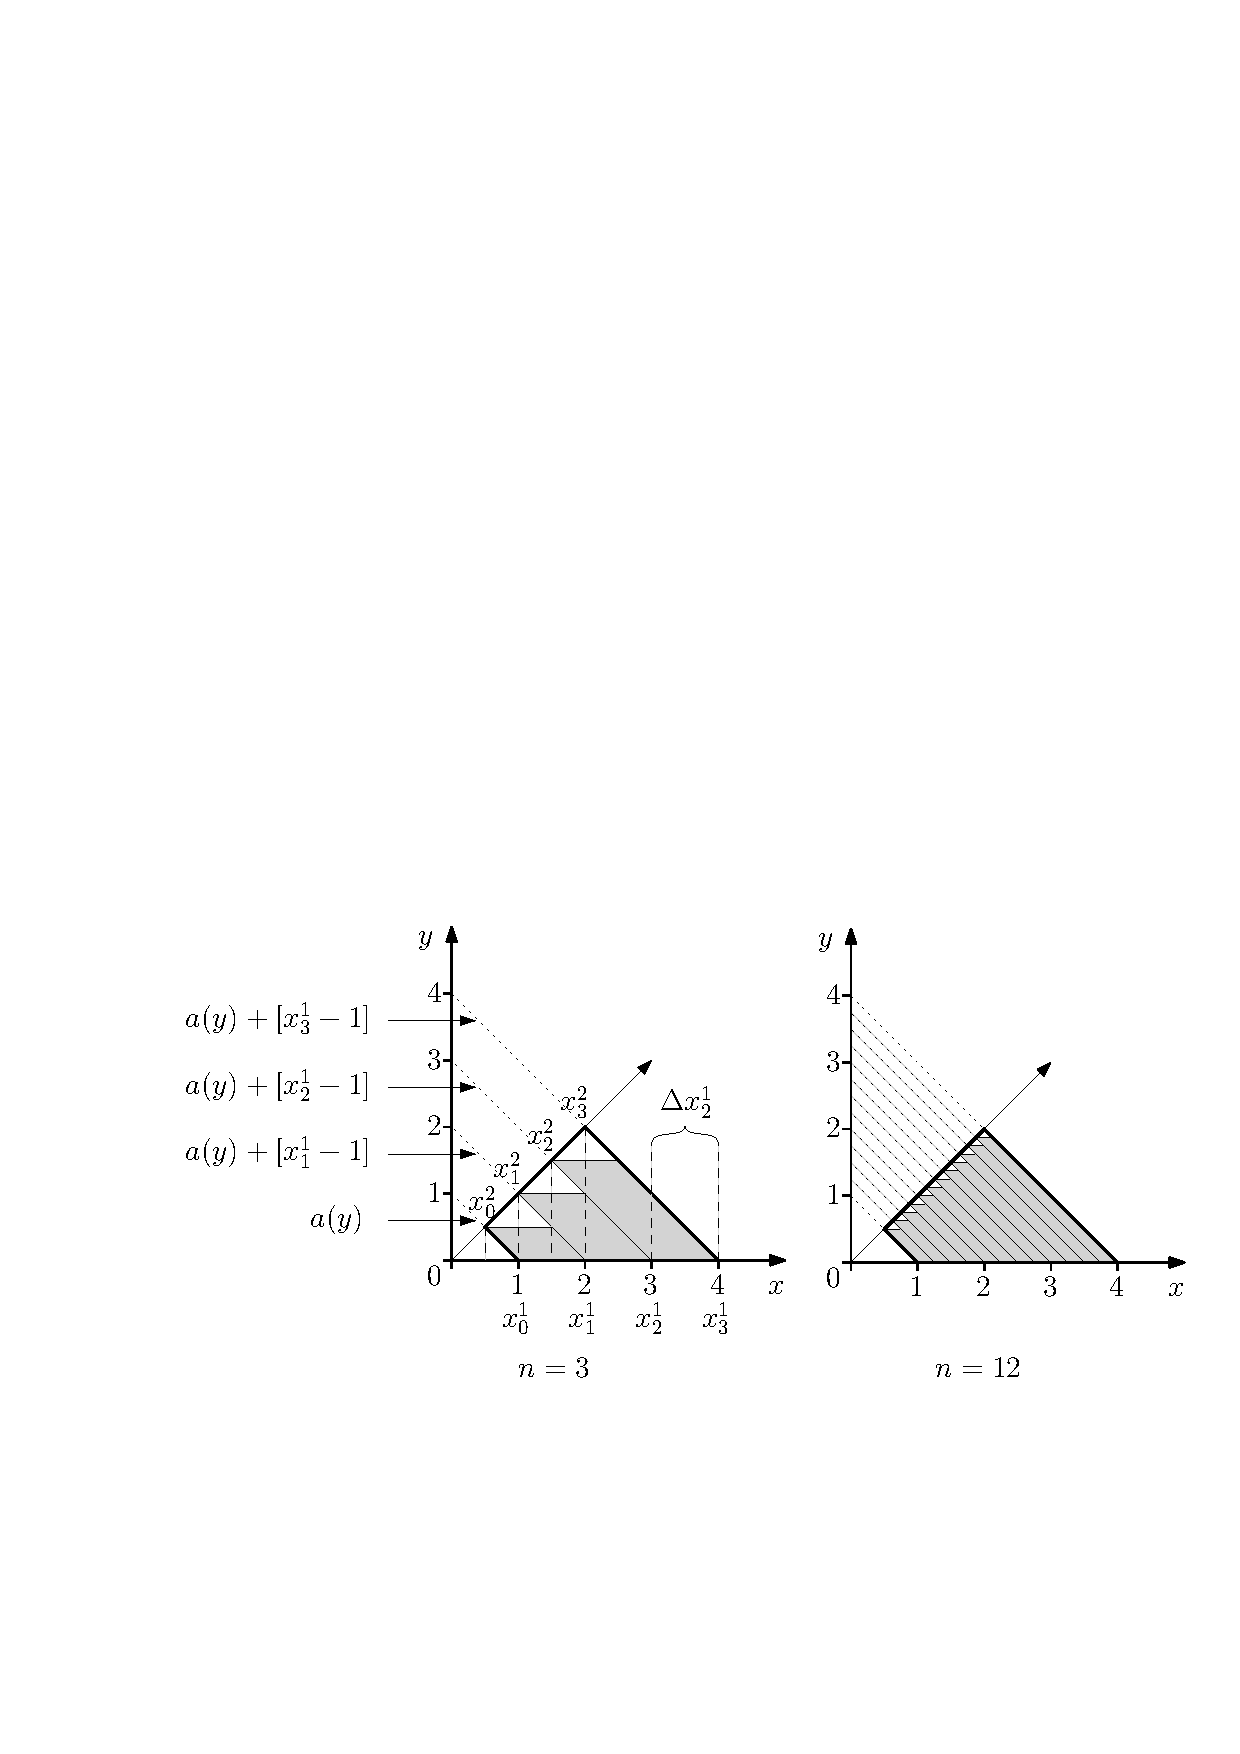
\includegraphics[width=0.75\textwidth]{fig13.pdf}
\caption{Region bounded by the $x$-axis and the lines $f(x)=x$, $a(y)=1-y$, and $b(y)=4-y$. In the case of $R$: $a=1$, $b=4$, $a'=\frac{1}{2}$ and $b'=2$. The figure also depicts the partition points $x_i^2$ as used in the Cavalieri sum (see Equation~\eqref{eq:cav_sum}). Reproduced from Quaestiones Mathematicae (2012) 35: 265-296 with permission \copyright~ NISC (Pty) Ltd.}
\label{fig:caval2}
\end{figure}

%\noindent
%The area of $R$ can be determined as follows if we employ the classical notion of integration:
%\begin{equation}
%\int_0^2x\, dx+\int_2^44-x\, dx- \int_0^{\frac{1}{2}}x\, dx-\int_{\frac{1}{2}}^11-x\, dx = 3.75. 
%\end{equation}

\noindent
We can approximate the area of $R$ by using rectangular integration strips. It, however, seems much more straightforward to approximate the area of $R$ via non-overlapping non-rectangular integration strips that toghether inscribe $R$. This can only be accomplished if the sides of the aforementioned integration strips are tranlsations of the function $a(y)$.\\

\noindent
Let us express this idea more formally. Let $(x_i^1)_{i=0}^{n}$ denote a partition on the $x$-axis, such that $a = x_0^1 < x_1^1 < \cdots < x_n^1 = b$, and $\Delta x_i^1 = x_{i+1}^1 - x_i^1$. We are now able to construct the following lower Cavalieri sum (see Equation~\ref{eq:c_low}):
\begin{equation}
\label{eq:cav_sum}
\sum_{i=0}^{n-1} f(x_i^2)\Delta x_i^1.
\end{equation}
The partition points $(x_i^2)_{i=0}^{n}$ are depicted in Figure~\ref{fig:caval2}. Cavalieri's principle tells us that the area of integration strip $i$ is equal to $f(x_i^2)\Delta x_i^1$. Equation.~\eqref{eq:cav_sum}, therefore, approximates the area of $R$. In the limit equation~\eqref{eq:cav_sum} approaches 
the Cavalieri integral (see Definition~\ref{def:cav_integral}):
\begin{equation}
\label{eq:caval1}
\int_{a(y)}^{b(y)}f(x)\, dx = \lim_{n\to \infty}\sum_{i=0}^{n-1} f(x_i^2)\Delta x_i^1.
\end{equation}
If we evaluate the above integral we obtain the area of $R$. It is, however, quite hard to evaluate the above integral in its present form. Fortunately, it is easy to convert a Cavalieri integral into an equivalent Riemann or Riemann-Stieltjes 
integral by using the functions $h$ and $g$ (see equation~\ref{eq:g_def} and equation~\ref{eq:h_def}). Expressed mathematically (see Theorem~\ref{t:conv}):
\begin{equation}
\label{eq:main_cav}
\int_{a(y)}^{b(y)}f(x)\,dx =\int_a^b f \circ h (x)\, dx = \int_{a'}^{b'} f(x) dg(x),
\end{equation}
We can, therefore, evaluate equation~\ref{eq:main_cav} in one of two ways:
\begin{equation}
\int_{a(y)}^{b(y)}f(x)\, dx = \int_a^b f \circ h (x)\, dx = \dfrac{1}{2}\int_1^4x\, dx = 3.75,  
\end{equation}
or
\begin{equation}
\int_{a(y)}^{b(y)}f(x)\, dx = \int_{a'}^{b'} f \, dg(x) = \int_{\frac{1}{2}}^2x\, d2x = 3.75.  
\end{equation}
Note, in the above two equations: $h(x) = \frac{1}{2}x$ and $g(x) = 2x$.\\ 

\noindent
We can easily verify that the above is correct:
\begin{equation}
\int_0^2x\, dx+\int_2^44-x\, dx- \int_0^{\frac{1}{2}}x\, dx-\int_{\frac{1}{2}}^11-x\, dx = 3.75. 
\end{equation}

%Recall from Section, that not every Riemann-Stieltjes integral $\int_{a'}^{b'} f(x) d\,\widetilde{g}(x)$ can directly be converted into a Cavalieri integral. We usually first need to convert it into an equivalent Riemann-Stieltjes integral $\int_{a'}^{b'} f(x) d\,g(x)$. The Riemann-Stieltjes integral so obtained can then be converted into a Cavalieri integral. The former conversion is achieved by computing the scalar $C$. Once, $C$ is known the latter conversion follows trivially (see Section).

\noindent
The natural question now arises, can we convert a Riemann-Stieltjes integral into a Cavalieri integral? As an example, can the following Riemann-Stieltjes integral be converted into a Cavalieri integral?
\begin{equation}
\int_{a'}^{b'} \,d\,\widetilde{g}(x) = \int_{\frac{1}{2}}^2 x\,d[2x+1].
\end{equation}
To accomplish this task we first need to compute the following (see Section~\ref{sec:cav_integral}):
\begin{itemize}
 \item $a(y) = f^{-1}(y) - \widetilde{g}\circ f^{-1}(y)+ \widetilde{g}(a') = 1-y$.
 \item $a = a(0) = 1$.
 \item $C = a - \widetilde{g}(a') = -1$.
 \item $g(x) = \widetilde{g}(x) + C = 2x$.
 \item $b = g(b') = 4$ and $b(y) = a(y) + (b-a) = 4-y$.
\end{itemize}
It now follows that:
\begin{equation}
\int_{a'}^{b'} f(x)d\,\widetilde{g}(x) = \int_{a'}^{b'} f(x)d\,g(x) := \int_{a(y)}^{b(y)} f(x)dx, 
\end{equation}
with $a(y) = 1-y$, $b(y) = 4-y$ and $C=-1$.

\section{Left-sided Riemann-Liouville Fractional Integral}
\noindent
For the sake of completeness, let us review the definition of the left-sided Riemann-Liouville fractional integral of order $\alpha$ (based at $a'$) \cite{laurent1884}. Let
\begin{equation}
_{a'}I_t\, f(t) := \int_{a'}^t f(\tau)~d\tau.
\end{equation}
Please note that in this paper from this point onwards our variable of integration will be $\tau$ instead of $x$. It is of our opinion that this notational change improves the readability of the paper (if $\tau$ is our variable of integration then it makes sense to choose $t$ as our upper integration limit).\\

\noindent
If we apply the above operator in a repetitive manner to $f$ we obtain the $n$th antiderivative of $f$ based at $a'$:
\begin{equation}
\label{eq:n_anti}
_{a'}I_t^n\,f(t) = \int_{a'}^t\int_{a'}^{\tau_1}\cdots \int_{a'}^{\tau_{n-1}}f(\tau_n)~d\tau_n\cdots d\tau_2 d\tau_1.
\end{equation}
Applying Cauchy's repetitive integration formula to equation~\eqref{eq:n_anti} results in:
\begin{equation}
\label{eq:cauchy}
_{a'}I_t^n\,f(t) = \frac{1}{(n-1)!}\int_{a'}^t (t-\tau)^{n-1}f(\tau)~d\tau.
\end{equation}
% As an example if $f(t)=t$, $n=2$ and $a'=0$ then equation~\eqref{eq:cauchy} reduces to:
% \begin{equation}
% _{0}I_t^2\,f(t) = \int_0^t (t-\tau)\tau~d\tau = \frac{\tau^2 t}{2} - \frac{\tau^3}{3} \Bigg |_0^t = \frac{t^3}{3!}.
% \end{equation}
The definition in equation~\eqref{eq:cauchy} can now be extended to an arbitrary fractional order by replacing $(n-1)!$ with the Gamma function (see Figure~\ref{fig:gamma}):
\begin{equation}
\label{eq:frac_integral}
_{a'}I_t^{\alpha}f(t) = \frac{1}{\Gamma(\alpha)}\int_{a'}^t (t-\tau)^{\alpha-1}f(\tau)~d\tau.
\end{equation}
Equation~\eqref{eq:frac_integral} is known as the left-sided Riemann-Liouville fractional integral of order $\alpha$. 
% As an example if $f(t)=t$, $\alpha=\frac{1}{2}$ and $a'=0$ then 
% equation~\eqref{eq:frac_integral} reduces to:
% \begin{equation}
% _0 I_t^{\frac{1}{2}}\,f(t) = \frac{1}{\Gamma(\frac{1}{2})} \int_0^t \frac{\tau}{\sqrt{t-\tau}} d\tau = \frac{1}{\sqrt{\pi}}\left [ -\frac{2}{3}\sqrt{t-\tau}(2t+\tau)\right] \Bigg |_0^t=\frac{4}{3\sqrt{\pi}}t^{\frac{3}{2}}. 
% \end{equation}

% \begin{figure}[htb]
% \centering
% 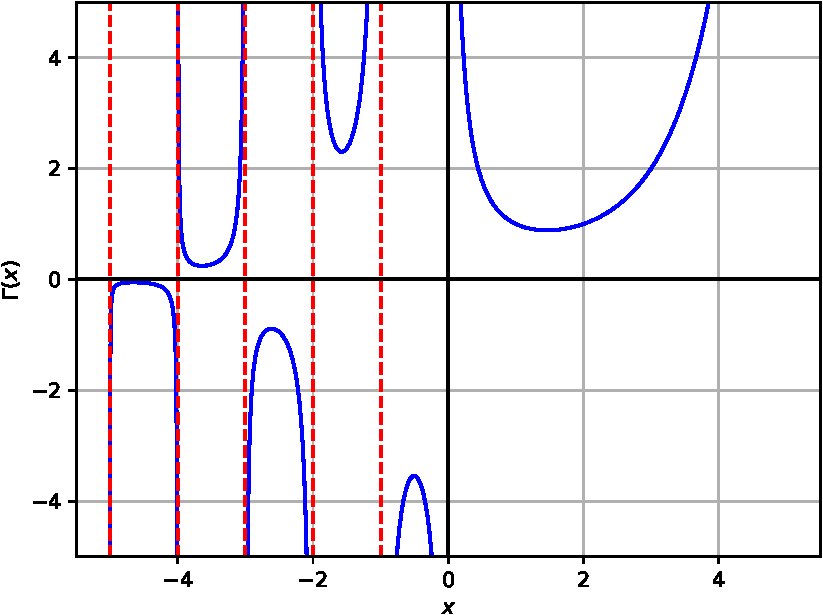
\includegraphics[width=0.7\textwidth]{gamma.pdf}
% \caption{A plot of $\Gamma(x) = \int_0^{\infty} t^{x-1} e^{-t}\,dt$ for $x\in(-5,5)$. $\Gamma(x)$ is not defined for the negative integers. Moreover, it is a natural extension of the factorial function to the real numbers \cite{euler1738}.}
% \label{fig:gamma}
% \end{figure}

\section{Geometric Interpretation of the Left-sided Riemann-Liouville Fractional Integral}

\subsection{Converting into a Riemann-Stieltjes integral}
Podlubny showed that the Left-sided Riemann-Liouville fractional integral can be converted into a Riemann-Stieltjes integral \cite{podlubny02}:

\begin{equation}
\label{eq:rl_to_rs}
_{a'}I_t^{\alpha}\,f(t) = \frac{1}{\Gamma(\alpha)}\int_{a'}^{t}(t-\tau)^{\alpha-1}f(\tau)~d\tau = \int_{a'}^{t} f(\tau)~d\,\widetilde{g}_t^{\alpha}(\tau), 
\end{equation}
with 
\begin{equation}
\label{eq:g_rl}
\widetilde{g}_t^{\alpha}(\tau) = \frac{\left \{t^{\alpha} - (t-\tau)^{\alpha} \right \}}{\Gamma(\alpha+1)}. 
\end{equation}
Moreover, the function $\widetilde{g}_t^{\alpha}(\tau)$ is invertable. Its inverse is:
\begin{equation}
\widetilde{h}_t^{\alpha}(\tau) = t - \sqrt[\alpha]{t^{\alpha} - \Gamma(\alpha+1)\tau}.
\end{equation}
The function $\widetilde{g}_t^{\alpha}$ is invertable, since $\frac{d \widetilde{g}_t^{\alpha}}{d\tau}=\frac{(t-\tau)^{\alpha-1}}{\Gamma(\alpha)} > 0$ for $\tau\in(-\infty,t]$. Let $\mathsf{A} = \{0,0.2,0.4,0.6,0.8,1\}$. The graphs of $\widetilde{g}_{10}^{\alpha}(\tau)$ and $\widetilde{h}_{10}^{\alpha}(\tau)$ are depicted in Figure~\ref{fig:gandh}.


%\begin{theorem}
%Let $C\in\mathbb{R}$. The following integrals are equivalent
%\end{theorem}

%\begin{proof}
%Note that 
%\begin{equation}
%\label{eq:diff}
%\frac{dg_t^{\alpha}(\tau)}{d\tau} = \frac{\alpha(t-\tau)^{\alpha-1}}{\Gamma(\alpha+1)} =%\frac{(t-\tau)^{\alpha-1}}{\Gamma(\alpha)}. 
%\end{equation}
%Furthermore,
%\begin{equation}
%\label{eq:inter_step}
%\int_{a'}^{t} f(\tau)\,dg_t^{\alpha}(\tau) = \int_{a'}^{t} f(\tau) \frac{dg_t^{\alpha}%(\tau)}{d\tau}\,d\tau. 
%\end{equation}
%The desired result is obtained by substituting Equation~\eqref{eq:diff} into Equation~\eqref{eq:inter_step}.  
%\end{proof}

%\begin{theorem}
%The function $g_t^{\alpha}(\tau)$ is invertable. Its inverse is:
%\begin{equation}
%h_t^{\alpha}(\tau) = t - \sqrt[\alpha]{t^{\alpha} - \Gamma(\alpha+1)(\tau-C)}.
%\end{equation}
%\end{theorem}
%\begin{proof}
% The inverse now follows trivially.  
%\end{proof}


% \begin{table}[h!]
%  \centering
%  \caption{The analytic expressions of $\widetilde{g}_{10}^{\alpha}(\tau)$ and $\widetilde{h}_{10}^{\alpha}(\tau)$ for $\alpha\in\mathsf{A}$. The expressions in this table are depicted in Fig~\ref{fig:gandh}.}
%  \label{tab:gandh}
%  \begin{tabular}{|c || c | c|} 
%  \hline 
%  \rule{0pt}{3ex}
%  $\alpha$ &  $\widetilde{g}_{10}^{\alpha}(\tau)$ & $\widetilde{h}_{10}^{\alpha}(\tau)$ \\
%  \hline\hline
%  $0$ & 0 & $y=0$ \\ 
%  $0.2$ & $[\Gamma\left (\frac{6}{5} \right )]^{-1}\left(\sqrt[5]{10}-\sqrt[5]{10-\tau}\right)$ & $10 - \left ( \sqrt[5]{10} -  \Gamma\left (\frac{6}{5} \right ) \tau \right )^5$  \\
%  $0.4$ & $[\Gamma\left (\frac{7}{5} \right )]^{-1}\left(\sqrt[5]{10^2}-\sqrt[5]{(10-\tau)^2}\right)$ & $10 - \sqrt{\left ( \sqrt[5]{10^2} -  \Gamma\left (\frac{7}{5} \right ) \tau \right )^5}$ \\
%  $0.6$ & $[\Gamma\left (\frac{8}{5} \right )]^{-1}\left(\sqrt[5]{10^3}-\sqrt[5]{(10-\tau)^3}\right)$ & $10 - \sqrt[3]{\left ( \sqrt[5]{10^3} -  \Gamma\left (\frac{8}{5} \right ) \tau \right )^5}$ \\
%  $0.8$ & $[\Gamma\left (\frac{9}{5} \right )]^{-1}\left(\sqrt[5]{10^4}-\sqrt[5]{(10-\tau)^4}\right)$ & $10 - \sqrt[4]{\left ( \sqrt[5]{10^4} -  \Gamma\left (\frac{9}{5} \right ) \tau \right )^5}$ \\ [1ex] 
%  $1$ & $\tau$ & $\tau$ \\ [1ex] 
%  \hline
%  \end{tabular}
%  \end{table}

\begin{figure}[htb]
\centering
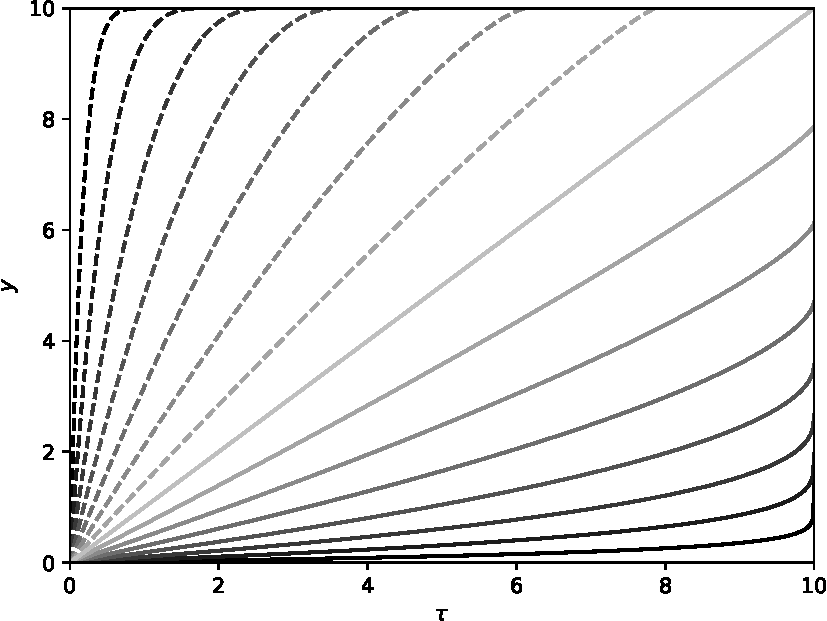
\includegraphics[width=0.75\textwidth]{gh.pdf}
\caption{This figure depicts the curves of $\widetilde{g}_{10}^{\alpha}(\tau)$ and $\widetilde{h}_{10}^{\alpha}(\tau)$ for $\alpha\in\mathsf{A}$. The curves associated with $\widetilde{g}$ are plotted using solid lines, while the curves plotted using dashed lines are associated with $\widetilde{h}$. The lighter the shade with which a curve is depicted, the larger the $\alpha$-value is that is associated with it.}
\label{fig:gandh}
\end{figure}

%\subsection{Podlubny's Geometric Interpretation}
\noindent
Podlubny also showed that we can assign a geometric meaning to the fractional integral in equation~\eqref{eq:rl_to_rs} by visualizing the equivalent Riemann-Stieltjes integral contained within the same equation using Bullock's geometric framework. Consider the axis $\tau$, $\widetilde{g}_t^{\alpha}$ and $f(\tau)$. Podlubny suggests that we build a ``fence'' in $(\tau,\widetilde{g}_t^{\alpha},f)$-space. The base of the aforementioned fence is given by the curve $(\tau,\widetilde{g}_t^{\alpha}(\tau),0)$, while its height is determined by $(\tau,\widetilde{g}_t^{\alpha}(\tau),f(\tau))$. The ``shadow'' of this fence, i.e. the area under the curve which is obtained by projecting this fence onto the $\widetilde{g}f$-plane corresonds to the value which is obtained when equation~\eqref{eq:rl_to_rs} is evaluated. As an example, the geometric interpretation so obtained for the integrand $f(t)=\sqrt{t}$ is depicted in Figure~\ref{fig:vis_old}.

%geometric idea is depicted in Fig for $f(t)=\sqrt{t}$, $\alpha\in\{0.3,0.6,0.9\}$ and $\t\in\{3,6,9\}$. 


\begin{figure}[htb]
\centering
\includegraphics[width=1.0\textwidth]{vis_old.pdf}
\caption{This figure depicts the visualization of $\frac{1}{\Gamma(\alpha)}\int_{0}^{t}(t-\tau)^{\alpha-1}\sqrt{\tau}~d\tau$ using the geometric framework proposed by Podlubny.
As is indicated in the figure, the graphs contained in each row of the subfigure-grid are obtained by varying $\alpha$, while the graphs contained in each column of the subfigure-grid are obtained by varying $t$. The fence itstelf is depicted in green. The areas depicted in red (the shadow of the fence) correspond to the value obtained when $\frac{1}{\Gamma(\alpha)}\int_{0}^{t}(t-\tau)^{\alpha-1}\sqrt{\tau}~d\tau$ is evaluated.  The surface which is obtained by extending the curve $f(\tau)$ and $\widetilde{g}_t^{\alpha}(\tau)$ along the $\widetilde{g}$ and $f$ direction is depicted in cyan and blue, respectively. The intersection between the blue and cyan 
surfaces represents the curve that determines the height of the aforementioned fence (and is depicted as a dashed curve).   
}
\label{fig:vis_old}
\end{figure}


\subsection{Converting into a Cavalieri integral}
\label{sec:rl_to_cav}
Recall that,
\begin{equation}
_{a'}I_t^{\alpha}\,f(t) = \frac{1}{\Gamma(\alpha)}\int_{a'}^{t}(t-\tau)^{\alpha-1}f(\tau)~d\tau = \int_{a'}^{t} f(\tau)~d\,\widetilde{g}_t^{\alpha}(\tau). 
\end{equation}
%Furthermore, note that for all $K\in\mathbb{R}$ (see Theorem~\ref{}):
%\begin{equation}
%\int_{a'}^{t} f(\tau)~d\,[\widetilde{g}_t^{\alpha}(\tau)+K] = \int_{a'}^{t} f(\tau)~d%\,\widetilde{g}_t^{\alpha}(\tau),  
%\end{equation}
%Moreover, let $C$ be a real-valued constant so that with $g_t^{\alpha}(\tau) = \widetilde{g}_t^{\alpha}(\tau) + C$. 
%Recall, if we wish to convert a Riemann-Stieltjes integral into a Cavalieri integral we normally first need to convert the given Riemann-Stieltjes integral into an equivalent 
%Riemann-Stieltjes integral which we can  by computing a value for $C$. This latter integral can then be converted into a Cavalieri integral. The steps that are required to perform this conversion in the case of Eq is presented below (see Section~\ref{}):
Let us first compute the following (see Section~\ref{sec:cav_integral}):
\begin{itemize}
 \item $a_t^{\alpha}(y) = f^{-1}(y) - \widetilde{g}_t^{\alpha}\circ f^{-1}(y)+ \widetilde{g}_t^{\alpha}(a')$.
 \item $a = a_t^{\alpha}(0)$.
 \item $C = a - \widetilde{g}_t^{\alpha}(a')$.
 \item $g_t^{\alpha}(\tau) = \widetilde{g}_t^{\alpha}(\tau) + C$.
 \item $b = g_t^{\alpha}(b')$ and $b_t^{\alpha}(y) = a_t^{\alpha}(y) + (b-a)$.
\end{itemize}
It now follows that:
\begin{equation}
\label{eq:rl_to_c}
_{a'}I_t^{\alpha}\,f(t) =  \frac{1}{\Gamma(\alpha)}\int_{a'}^{t}(t-\tau)^{\alpha-1}f(\tau)~d\tau= \int_{a'}^{t} f(\tau)~dg_t^{\alpha}(\tau) := \int_{a_t^{\alpha}(y)}^{b_t^{\alpha}(y)} f(\tau)\,d\tau.
\end{equation}

\noindent
Let $R_t^{\alpha}$ denote the region which is bounded by $a_t^{\alpha}(y)$, $b_t^{\alpha}(y)$, $f(t)$ and the $\tau$-axis. Moreover, let $A_{t}^{\alpha}$ denote the area of $R_t^{\alpha}$. Equation~\ref{eq:rl_to_c} implies that when we evaluate $_{a'}I_t^{\alpha}\,f(t)$ we obtain $A_{t}^{\alpha}$. In other words, when we evaluate equation~\ref{eq:rl_to_c} we are actually summing together the area of an infinite number of non-rectangular infinitesimals inscribing $R_t^{\alpha}$. The aforementioned infinitesimals are, however, non-static, since they need to be translations of $a(y)_t^{\alpha}$. The shape of these infitesimals are thus dependend on $\alpha$ and $t$. In summary, we can obtain a novel geometric interpretation of 
$_{a'}I_t^{\alpha}\,f(t)$ by first converting it into a Cavalieri integral. We will take the liberty in this paper to refer to the depiction of the aformentioned Cavalieri integral as the non-static non-rectangular sum-based geometric interpretation of $_{a'}I_t^{\alpha}\,f(t)$.\\

%Stated differently, we can approximate $_{a'}I_t^{\alpha}\,f(t)$ via a Cavalieri sum, the shape of the integration strips used within this sum will be determined by $a_t^{\alpha}(y)$. In the limit this sum approaches $_{a'}I_t^{\alpha}\,f(t)$. The value $_{a'}I_t^{\alpha}\,f(t)$ so obtained is equal to the area of $R_t^{\alpha}$. $R_t^{\alpha}$ can, therefore, be decomposed into an infinite number of infinitesimals, each one of them being a translation of $a_t^{\alpha}(y)$. The shape of the aforementioned infenitesimals are non-static, since their shape depend on the value of $t$ and $\alpha$.

\noindent
Let $h_t^{\alpha}(\tau)$ be equal to the inverse of $g_t^{\alpha}(\tau)$. Interestingly, Theorem~\ref{t:conv} implies that we can use $h_t^{\alpha}(\tau)$ to convert equation~\eqref{eq:rl_to_c} into the following Riemann integral:
\begin{equation}
\label{eq:rl_to_r}
\int_{g_t^{\alpha}(a')}^{\frac{t^{\alpha}}{\Gamma(\alpha+1)}+C} f\circ h_{\alpha}^t (\tau) d\tau.  
\end{equation}
We can, therefore, evaluate equation~\eqref{eq:frac_integral} in one of two ways: we can either evaluate equation~\eqref{eq:rl_to_rs} or we can evaluate equation~\eqref{eq:rl_to_r}.

\subsection{Examples}
Consider the following fractional integral:
\begin{equation}
\label{eq:ex1_raw}
_0I_t^{\alpha} f(t) = \frac{1}{\Gamma(\alpha)}\int_0^t f(\tau) (t-\tau)^{\alpha-1}~d\tau = \frac{1}{\Gamma(\alpha)}\int_0^t \tau(t-\tau)^{\alpha-1}~d\tau. 
\end{equation}
The function $f(t) = t$ is depicted in Figure~\ref{fig:geo1}. We can now convert the above fractional integral into a Cavalieri integral (see Section~\ref{sec:rl_to_cav}):
\begin{equation}
\label{eq:ex1}
_0I_t^{\alpha} f(t) = \int_0^t f(\tau)~d\,\widetilde{g}_t^{\alpha}(\tau)=\int_0^t f(\tau)~d\,g_t^{\alpha}(\tau):=\int_{a_t^{\alpha}(y)}^{b_t^{\alpha}(y)} f(\tau)~d\tau,
\end{equation}
with $a_t^{\alpha}(y) = y - \frac{t^{\alpha}-(t-y)^{\alpha}}{\Gamma(\alpha+1)}$, $b_t^{\alpha}(y) = a_t^{\alpha}(y) + \frac{t^{\alpha}}{\Gamma(\alpha+1)}$ and $C=0$.
Note, that for this example $a'=a=0$. The non-static non-rectangular sum-based geometric interpretation associated with equation~\ref{eq:ex1} is depicted in Figure~\ref{fig:geo1} (see Section~\ref{sec:rl_to_cav}). We elaborate on this below.\\  

\begin{figure}[htb]
\centering
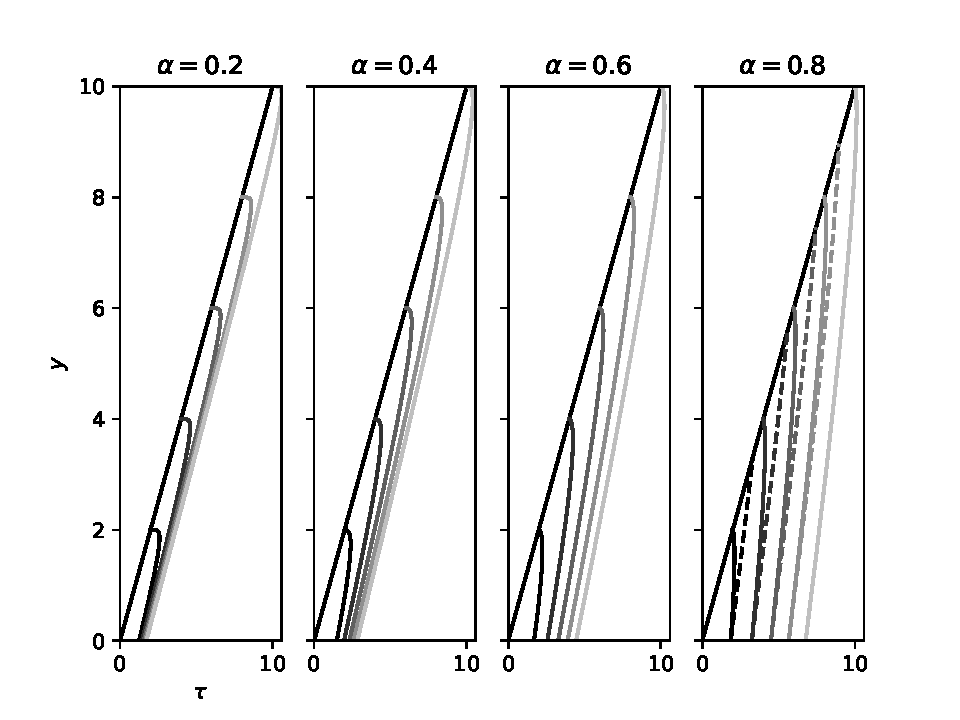
\includegraphics[width=0.75\textwidth]{geo_int1.pdf}
\caption{The non-static non-rectangular sum-based geometric interpretation of equation~\eqref{eq:ex1_raw}.}
\label{fig:geo1}
\end{figure}

% \noindent
% Since equation~\eqref{eq:ex1}, is a Cavalieri integral it has a known geometric interpretation (see Figure~\ref{fig:caval2}). It can be interpreted as the area obtained by summing together the areas of an infinite 
% number of infinitesimals whose shape is determined by $\alpha$ and $t$, i.e. these infinitesimals have to be translations of $b_t^{\alpha}(y)$. The geometric interpretation of equation~\eqref{eq:ex1_raw} is, therefore, non-static as it depends on the value of $\alpha$ and $t$. 
% There is one thing, however, which remains unclear: in what way do $\alpha$ and $t$ affect the shape of the aforementioned infinitesimals, i.e. how does the value of $\alpha$ and $t$ affect the shape of $b_t^{\alpha}(y)$. 
% We will answer this question by working through a detailed example.\\

%using two basic steps. First off, we will fix the value of $\alpha$ and $t$ in equation~\eqref{eq:ex1} and then depict $b_t^{\alpha}(y)$. We will then explore how varying the value of $\alpha$ and $t$ in equation~\eqref{eq:ex1} affects the shape $b_t^{\alpha}(y)$.\\
%We know that a Cavalieri integral can be interpreted as the area which is obtained by summing together the area associated with an infinite number of non-rectangular infinitesimals whose shape 
%is determined by the integration limits of the Cavalieri integral. Note that neither $g_t^{\alpha}(\tau)$ nor $a_t^{\alpha}(y)$ are static functions, 
%they depend on the value of $\alpha$ and $t$. This implies that a fractional integral of order $\alpha$ and extent $t$ can be interpeted as the area obtained by summing together the area associated with an infinite number of infinitesimals whose 
%shape is determined by $\alpha$ and $t$, i.e. the geometric interpretation of equation~\eqref{eq:ex1_raw} is non-static as it depends on the value of $\alpha$ and $t$.

% \noindent
% If we set the value of $\alpha$ to $\sfrac{4}{5}$ and the value of $t$ to 10 in equation~\eqref{eq:ex1} we obtain:
% \begin{equation}
% \label{eq:ex1_specific}
% _0I_{10}^{\sfrac{4}{5}} f(t) = \int_{a_{10}^{\sfrac{4}{5}}(y)}^{b_{10}^{\sfrac{4}{5}}(y)} f(\tau)~d\tau = A_{10}^{\sfrac{4}{5}}. 
% \end{equation}
% Let $R_{10}^{\sfrac{4}{5}}$ denote the region which is bounded by the $\tau$-axis, the function $f(\tau)$ and the function $b_{10}^{\sfrac{4}{5}}(y)$. The region $R_{10}^{\sfrac{4}{5}}$ is depicted in the right-most panel of Figure~\ref{fig:geo1}. It is the largest of all the regions depicted in the right-most panel of Figure~\ref{fig:geo1}. Moreover, let $A_{10}^{\sfrac{4}{5}}$ denote the area of $R_{10}^{\sfrac{4}{5}}$. When we evaluate Equation~\ref{eq:ex1_specific} we obtain $A_{10}^{\sfrac{4}{5}}$ (see Section~\ref{sec:rl_to_cav}). The region $R_{10}^{\sfrac{4}{5}}$ is not bounded by $a_{10}^{\sfrac{4}{5}}(y)$, since $a'=a=0$. Furthermore, note that the dashed grey-tinted curves in the right-most panel of Figure~\ref{fig:geo1} are translations of $b_{10}^{\sfrac{4}{5}}(y)$.\\

% We can approximate the area of $R_{10}^{\sfrac{4}{5}}$ by summing together the area of $n$ equal width non-rectangular integration strips that inscribe $R_{10}^{\sfrac{4}{5}}$, i.e. we can 
% construct a Cavalieri sum (see equation~\eqref{eq:cav_sum}). Note, the sides of the non-rectangular integration strips we use in this approximation have to be translations of $b_{10}^{\sfrac{4}{5}}(y)$.
% If we take the limit of the aforementioned sum as $n\rightarrow \infty$ we approach the Cavalieri integral in equation~\eqref{eq:ex1_specific}, i.e. $A_{10}^{\sfrac{4}{5}}$.  
% equation~\eqref{eq:ex1_specific}, therefore, implies that the region $R_{10}^{\sfrac{4}{5}}$ is made up 
% of an infinite number of non-rectangular infinitesimals; all of them being translations of $b_{10}^{\sfrac{4}{5}}(y)$. Note, the right-most curve depicted in the right-most panel of Figure~\ref{fig:geo1} is $b_{10}^{\sfrac{4}{5}}(y)$.  Moreover, the special case in which we approximate $A_{10}^{\sfrac{4}{5}}$ using five equal width non-rectangular integration strips is depicted in the right-most panel of Figure~\ref{fig:geo1}. 
% The sides of the aforementioned five integration strips are depicted in Figure~\ref{fig:geo1} using dashed lines. Let, $\mathcal{B}_{\mathsf{T}}^{\sfrac{4}{5}}=\{b_{10}^{\sfrac{4}{5}}(y)-c|c\in(\mathsf{T}-2)\}$ with $\mathsf{T}=\{2,4,6,8,10\}$.\\ 

%We have thus verified that we can employ the Cavalieri integral in equation~\eqref{eq:ex1_specific} to compute $A_{10}^{\sfrac{4}{5}}$ from first principles.
%Let $\mathsf{B}_{10}^{\sfrac{4}{5}}$ denote the set containing these dashed curves.
%We can, therefore, interpet equation~\eqref{}  The region $R_{10}^{\sfrac{4}{5}}$ is, therefore, made up 
%of an infinite number of non-rectangular infinitesimals; all of them being translations of $b_{10}^{\sfrac{4}{5}}(y)$.

\noindent
Let $\mathsf{T}=\{2,4,6,8,10\}$ and $\mathsf{A} = \{0,0.2,0.4,0.6,0.8,1\}$. Moreover, Let $R_{t}^{\alpha}$ denote the region which is bounded by the $\tau$-axis, the function $f(\tau)$ and the function $b_{t}^{\alpha}(y)$. Note that $b_{t}^{\alpha}(y)$ forms the 
right-most edge of $R_{t}^{\alpha}$. The region $R_{t}^{\alpha}$ is not bounded by $a_{t}^{\alpha}(y)$, since $a'=a=0$. Moreover, let $A_{t}^{\alpha}$ denote the area of $R_{t}^{\alpha}$ and let $\mathsf{R}_{\mathsf{T}}^{\mathsf{A}}=\{R_t^{\alpha}|t\in\mathsf{T},~\alpha\in\mathsf{A}\}$. The regions in the set $\mathsf{R}_{\mathsf{T}}^{\mathsf{A}}$ are depicted in Figure~\ref{fig:geo1}. The regions that are depicted in each of the panels of Figure~\ref{fig:geo1} were generated by varying $t$, whilst keeping the value of $\alpha$ fixed. The title of each panel indicates which $\alpha$-value was used to generate the regions depicted in each panel. The only difference between the regions located in each panel is their right edges. The right edges of the regions in each panel are depicted using varying shades of gray. The lighter the shade with which an edge is depicted, the larger the $t$-value is that is associated with it.\\

\noindent
We can interpret equation~\eqref{eq:ex1} as the value which is obtained when we sum together the area of an infinite number of non-rectangular infinitesimals inscribing $R_{t}^{\alpha}$. The value so obtained is $A_{t}^{\alpha}$ (see Section~\ref{sec:rl_to_cav}). Note that, the infinitesimals that are used in the aformentioned sum are translations of $R_{t}^{\alpha}$'s right edge. The following observations can now be made by inspecting Figure~\ref{fig:geo1}: 
\begin{description}
 \item[Effect of $\alpha$] the gray-tinted solid curves depicted in the different panels of Figure~\ref{fig:geo1} are not equal to one another, i.e. $b_{t}^{\alpha_1}(y)\neq b_{t}^{\alpha_2}(y)$ when $\alpha_1\neq\alpha_2$. 
 \item[Effect of $t$] Note that the dashed grey-tinted curves in the right-most panel of Figure~\ref{fig:geo1} are translations of $b_{10}^{\sfrac{4}{5}}(y)$. The dashed gray-tinted curves and the solid gray-tinted curves in the right-most panel are not equal to one another. The gray-tinted solid curves depicted in each of the panels of Figure~\ref{fig:geo1} are, therefore, not translations of one another. 
\end{description}
The following can thus be concluded: the value of both $\alpha$ and $t$ alters the shape of the aforementioned infinitesimals. Interestingly, their shape is more affected by $\alpha$ than by $t$. The curves in Figure~\ref{fig:geo1} that are associated with the infinitesimals obtained by varying $t$, whilst keeping the value of $\alpha$ fixed are very similar in nature and there exists a high degree of correlation between the aforementioned curves (if their 
sizes are ignored). The curves in Figure~\ref{fig:geo1} associated with the infinitesimals obtained by varying $\alpha$, whilst keeping the value of $t$ fixed are quite different from one another (the aforementioned curves are not correlated).\\  

%In the case of $\alpha$: the gray-tinted solid curves depicted in each panel are not equal to one-another. Similarly, in the case of $t$: the dashed gray curves and the solid gray-tinted curves in the right-most panel are not equal to one-another, i.e.$\mathsf{B}_T^{\alpha}\neq\mathcal{B}_T^{\alpha}$.

% \begin{table}[h!]
% \centering
% \caption{Curves obtained by evaluating equation~\eqref{eq:ex1} and equation~\eqref{eq:ex2} for all $\alpha\in \mathsf{A}$ using either equation~\eqref{eq:rs} or equation~\eqref{eq:option2}.}
% \label{tab:eval}
% \begin{tabular}{||c|| c| c||} 
%  \hline
%  $\alpha$ & $\frac{1}{\Gamma(\alpha)}\int_0^t \tau(t-\tau)^{\alpha-1}~d\tau$ & $\frac{1}{\Gamma(\alpha)}\int_0^t \sqrt{\tau}(t-\tau)^{\alpha-1}~d\tau$ \\[0.5ex]
%  \hline\hline
%  \rule{0pt}{2.5ex}
%  $0$ & $t$ & $\sqrt{t}$  \\  
%  \rule{0pt}{2.5ex}
%  $0.2$ & $\frac{25}{6\Gamma(\frac{1}{5})} t^{\sfrac{6}{5}}$  & $\frac{\sqrt{\pi}}{2\Gamma(\frac{17}{10})} t^{\sfrac{7}{10}}$  \\ 
%  \rule{0pt}{2.5ex}
%  $0.4$ & $\frac{25}{14\Gamma(\frac{2}{5})} t^{\sfrac{7}{5}}$  & $\frac{\sqrt{\pi}}{2\Gamma(\frac{19}{10})} t^{\sfrac{9}{10}}$  \\
%  \rule{0pt}{2.5ex}
%  $0.6$ & $\frac{25}{24\Gamma(\frac{3}{5})} t^{\sfrac{8}{5}}$  & $\frac{\sqrt{\pi}}{2\Gamma(\frac{21}{10})} t^{\sfrac{11}{10}}$  \\ 
%  \rule{0pt}{2.5ex}
%  $0.8$ & $\frac{25}{36\Gamma(\frac{4}{5})} t^{\sfrac{9}{5}}$  & $\frac{\sqrt{\pi}}{2\Gamma(\frac{23}{10})} t^{\sfrac{13}{10}}$  \\ 
%  \rule{0pt}{2.5ex}
%  $1$ & $\frac{1}{2}t^2$  & $\frac{2}{3}t^{\sfrac{3}{2}}$  \\ [1ex]
%  \hline
%  \end{tabular}
% \end{table}

\begin{figure}[htb]
\centering
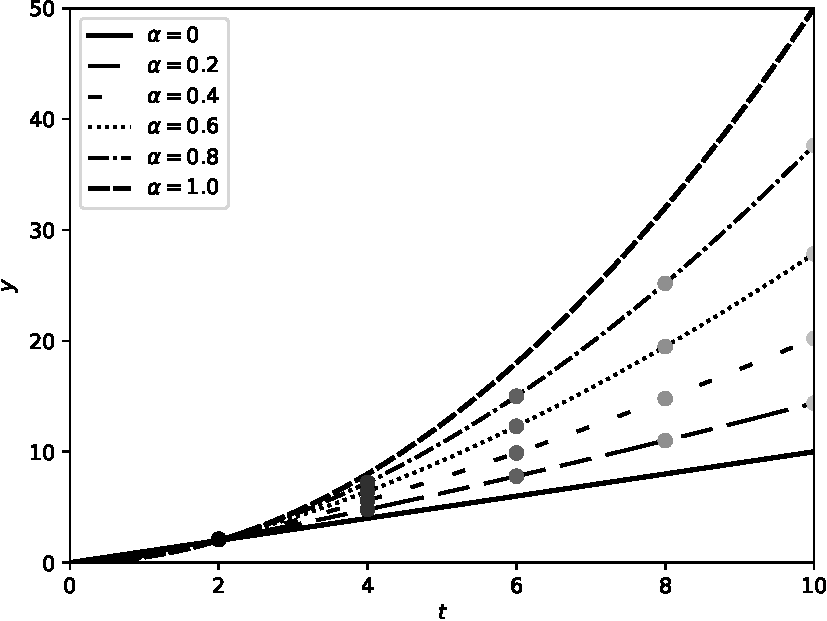
\includegraphics[width=0.75\textwidth]{func_eval1.pdf}
\caption{Depicts the curves which are obtained by evaluating equation~\eqref{eq:ex1} for all $\alpha\in \mathsf{A}$ using either equation~\eqref{eq:rs} or equation~\eqref{eq:option2}.}
\label{fig:eval1}
\end{figure}

\noindent
If we evaluate the integral in equation~\eqref{eq:ex1} for all $\alpha\in \mathsf{A}$ (using either equation~\eqref{eq:rl_to_rs} or equation~\eqref{eq:rl_to_r}) we obtain the curves depicted in in Figure~\ref{fig:eval1}. The area of the regions depicted in Figure~\ref{fig:geo1} are also plotted in Figure~\ref{fig:eval1} using circular markers. As expected, the circular markers in Figure~\ref{fig:eval1} that correspond to the areas of the regions in Figure~\ref{fig:eval1} associated with a particular choice of $\alpha$ (i.e. regions depicted in a particular panel of Figure~\ref{fig:geo1}) fall on the curve in Figure~\ref{fig:eval1}; associated with the same choice of $\alpha$. Moreover, note that we have adopted the same coloring scheme in Figure~\ref{fig:geo1} and Figure~\ref{fig:eval1}. Using the same coloring scheme in both figures makes it clear which of the area values in Figure~\ref{fig:eval1} can be associated with which regions in Figure~\ref{fig:geo1}. The validity of the geometric interpretation depicted in Figure~\ref{fig:geo1} is, therefore, corroborated by Figure~\ref{fig:eval1}. \\
%To summarize, Figure~\ref{fig:geo1}, therefore, depicts a non-static non-rectangular infinitesimal-based geometric interpretation of equation~\eqref{eq:ex1}. Moreover, Figure~\ref{fig:eval1} corroborates this geometric interpretation.\\

\noindent
Let us now consider a different fractional integral:
\begin{equation}
\label{eq:ex2}
\frac{1}{\Gamma(\alpha)}\int_0^t f(\tau) (t-\tau)^{\alpha-1}~d\tau = \frac{1}{\Gamma(\alpha)}\int_0^t \sqrt{\tau}(t-\tau)^{\alpha-1}~d\tau. 
\end{equation}
We can now convert the above fractional integral into a Cavalieri integral (see Section~\ref{sec:rl_to_cav}):
\begin{equation}
\label{eq:ex2_cav}
_0I_t^{\alpha} f(t) = \int_0^t f(\tau)~d\,\widetilde{g}_t^{\alpha}(\tau)=\int_0^t f(\tau)~d\,g_t^{\alpha}(\tau)=\int_{a_t^{\alpha}(y)}^{b_t^{\alpha}(y)} f(\tau)~d\tau,
\end{equation}
with $a_t^{\alpha}(y) = y^2 - \frac{t^{\alpha}-(t-y^2)^{\alpha}}{\Gamma(\alpha+1)}$, $b_t^{\alpha}(y) = a_t^{\alpha}(y) + \frac{t^{\alpha}}{\Gamma(\alpha+1)}$ and $C=0$.
Note, that for this example $a'=a=0$. The non-static non-rectangular sum-based geometric interpretation associated with equation~\ref{eq:ex2_cav} is depicted in Figure~\ref{fig:geo2} (see Section~\ref{sec:rl_to_cav}).

\begin{figure}[htb]
\centering
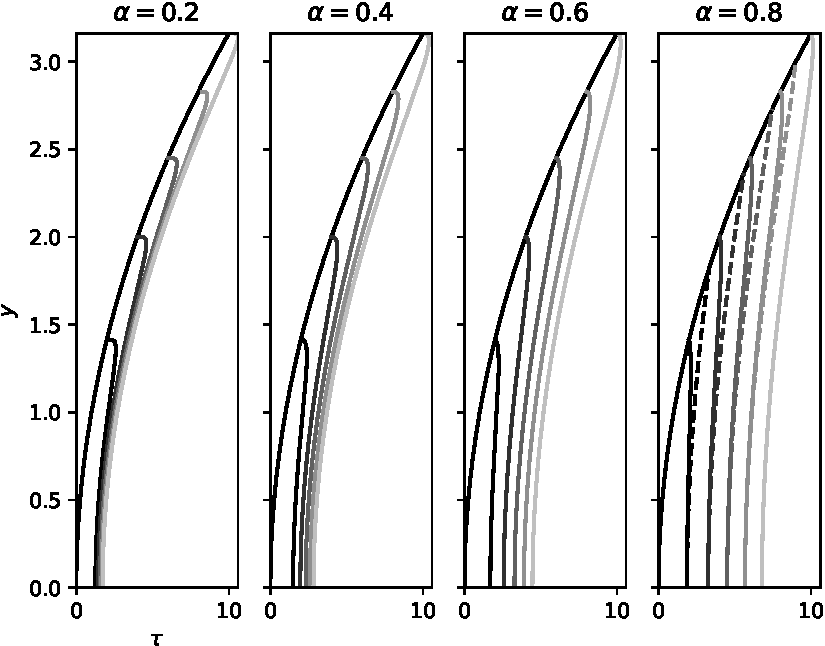
\includegraphics[width=0.75\textwidth]{geo_int2.pdf}
\caption{The non-static non-rectangular sum-based geometric interpretation of equation~\eqref{eq:ex2}.}
\label{fig:geo2}
\end{figure}

\section{Conclusion}
In this paper we presented a novel geometric interpretation of the left-sided 
Riemann-Liouville fractional integral. It can be interpreted as the value which is 
obtained by summing toghether the area of an infinite number of non-static non-rectangular infinitesimals. The shape of the infinitesimals used within the aforementioned sum depend on the order and the upper integration limit of the fractional integral under consideration.


%\begin{figure}[htb]
%\centering
%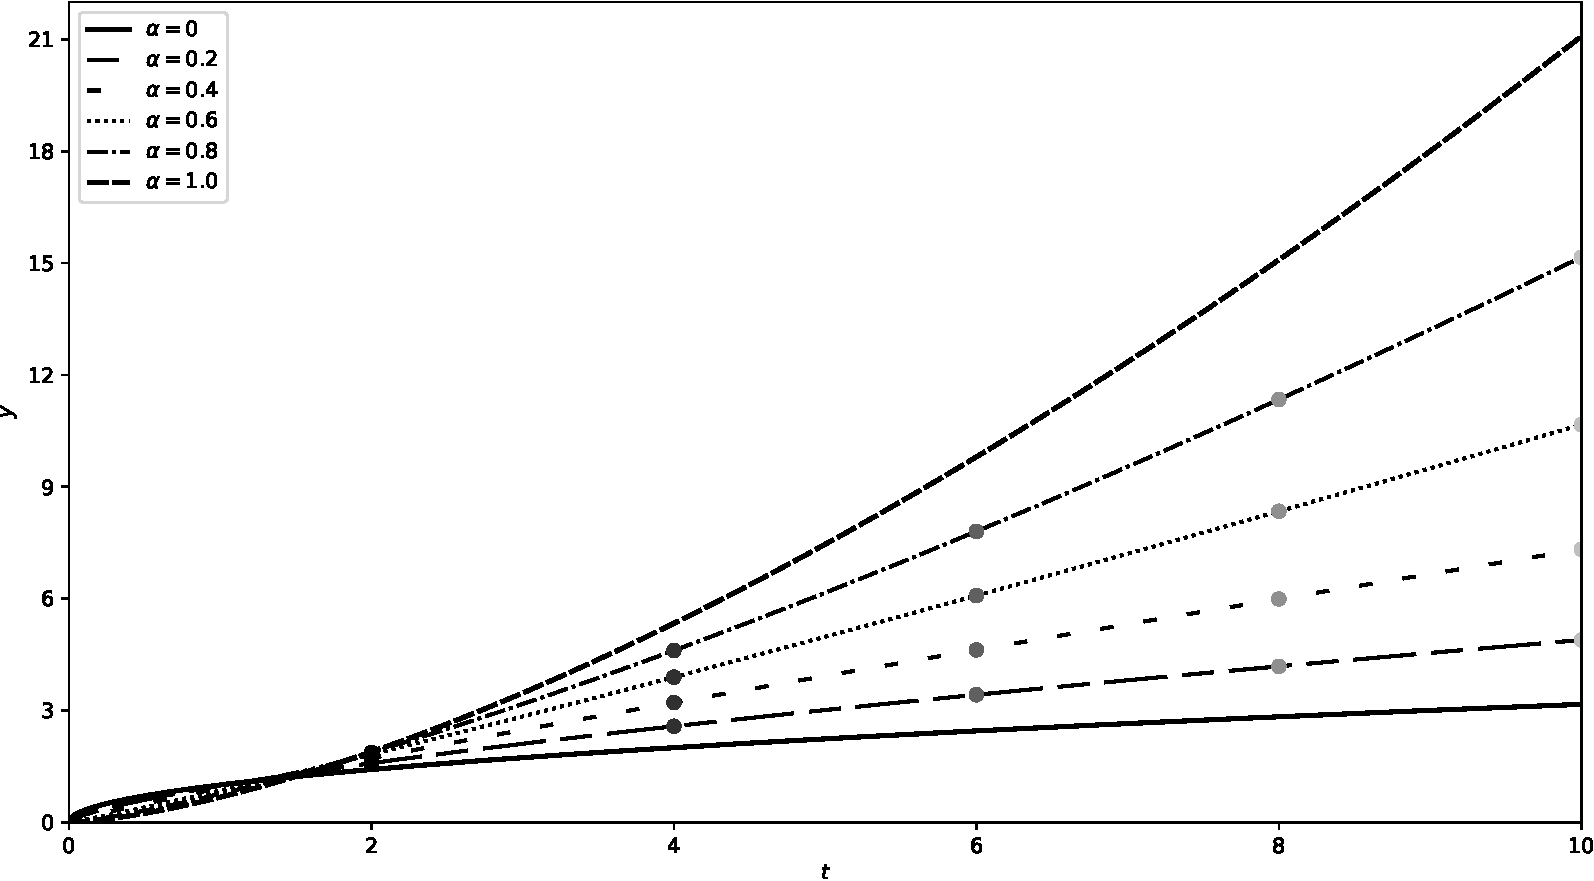
\includegraphics[width=0.75\textwidth]{func_eval2.pdf}
%\caption{Depicts the curves which are obtained by evaluating equation~\eqref{eq:ex2} %for all $\alpha\in \mathsf{A}$ using either equation~\eqref{eq:rs} or equation~\eqref{eq:option2}.}
%\label{fig:eval2}
%\end{figure}

%%%%%%%%%%%%%%%%%%%%%%%%%%%%%%%%%%%%%%%%%%%%%%%%%
%\section*{Acknowledgements}

% The author thanks his institution for the support, under Grant No ...

%%%%%%%%%% References %%%%%%%%%%%%%%%%%%%%%%%%%%%%%%%%
%%%% arranged in ALPHABETIC ORDER of Authors' Families
%%%% for articles, insert also DOI numbers if available

 \begin{thebibliography}{99}
 \normalsize
 
\bibitem{ackermann12} E.R.~Ackermann, T.L~Grobler, W.~Kleynhans,~W., J.C.~ Olivier, B.P.~Salmon, A.J.~van Zyl. Cavalieri
Integration. \textit{Quaest. Math.} \textbf{35}, No 3 (2012), 265--296.

\bibitem{adda97} F.B.~Adda, (1997). Geometric interpretation of the fractional derivative. \textit{J. of Fract. Calc.} \textbf{11}, (1997), 21--52.

\bibitem{bullock88} G.L.~Bullock. A geometric interpretation of the Riemann-Stieltjes integral. \textit{Am. Math. Mon.} \textbf{95}, No 5 (1988), 448--455.

%\bibitem{bartle76} R.G.~Bartle, \textit{The Elements of Real Analysis.} Wiley, New York (1976).

%Physical
%\bibitem{cioc16} Cioc, R. (2016). Physical and geometrical interpretation of Gr\"{u}nwald-Letnikov differintegrals: Measurement of path and acceleration. \textit{Fract. Calc. Appl. Anal.} 19(1): 161--172.

%\bibitem{davis59} Davis,~P.~J. (1959). Leonhard Euler's Integral: A Historical Profile of the Gamma Function. \textit{Amer. Math. Monthly}. 66(10): 849--869

%\bibitem{euler1738} Euler,~L. (1738). De progressionibus transcendentibus seu quarum termini generales algebraice dari nequeunt. \textit{Commentarii academiae scientiarum Petropolitanae}. 36--57.

\bibitem{garcia2019} J.P.~Garc\'{i}a-Sandoval, On representation and interpretation of Fractional calculus and fractional order systems. \textit{Fract. Calc. Appl. Anal.}, \textbf{22}, No 2 (2019), 522---537.

%\bibitem{gomez14} J.F~Gomez-Aguilara, R.~Razo-Hernandez, D.A.~Granados-Lieberman. Physical interpretation of fractional
%calculus in observable terms: analysis of the fractional time constant and the transitory response. \textit{Revista Mexicana de Fisica.} \textbf{60}, (2014), 32--38.

\bibitem{grobler19} T.L.~Grobler. Visualization of the Riemann-Stieltjes integral. \textit{Coll. Math. J.} \textbf{50}. No 3 (2019), 198--209.

\bibitem{laurent1884} H.~Laurent, (1884). Sur le calcul des d\'{e}riv\'{e}es \`{a} indices quelconques. \textit{Nouv Annales de Mathem\'{e}matiques.} \textbf{3}, No 3 (1884), 240--252. 

%\bibitem{liouville1832} Liouville,~J. (1832). M\'{e}moire sur l\textquotesingle integration de l\textquotesingle \'{e}quation $(mx^2+nx+p)\frac{d^2y}{dx^2}+(qx+r)\frac{dy}{dx}+sy$ \`{a} l\textquotesingle aide des diff\'{e}rentielles \`{a} indices 
%que\textquotesingle conques. \textit{Journal d l\textquotesingle Ecole Polytechnique.} 13(21): 163--186. 

\bibitem{machado03} J.T.~Machado. A probabilistic interpretation of the fractionalorder differentiation. \textit{Fract. Calc. Appl. Anal.} \textbf{6}, No 1 (2003), 73--80.

%\bibitem{machado14} Machado,~J.~T., Galhano,~A.~M., Trujillo,~J.~J. (2014). On development of fractional calculus during the last fifty years. \textit{Scientometrics}. 98(1): 577-582.

\bibitem{machado17} J.T.~Machado, V.~Kiryakova. The chronicles of fractional calculus. \textit{Fract. Calc. Appl. Anal.} \textbf{20}, No 2 (2017), 307--336.

%\bibitem{munkhammar05} Munkhammar,~J. (2005). Fractional calculus and the Taylor-Riemann series. \textit{Rose-Hulman Undergrad. Math. J.}, 6(1): 6.

%physical
\bibitem{nigmatullin92} R.R.~Nigmatullin. A fractional integral and its physical interpretation. \textit{Theor. and Math. Phys.} \textbf{90}, No 3 (1992): 242--251.

\bibitem{podlubny02} Podlubny,~I. Geometric and Physical Interpretation of Fractional Integration and Fractional Differentiation, \textit{Fract. Calc. Appl. Anal.} \textbf{5}, No 4 (2002), 367--386.

%\bibitem{riemann1876} Riemann,~B.~G.~F (1876). Gesammelte Werke.

%\bibitem{ross77} Ross,~B. (1977). The development of fractional calculus 1695--1900. \textit{Hist. Math.} 4(1): 75--89.

\bibitem{ross06} B.Ross, (Ed.). \textit{Fractional calculus and its applications: proceedings of the international conference held at the University of New Haven, June 1974}, \textbf{457}, Springer (1974).
 
\bibitem{rutman95} R.S.~Rutman. On physical interpretations of fractional integration and differentiation. \textit{Theor. and Math. Phys.} \textbf{105}, No 3 (1994),1509--1519.

 %Probability
\bibitem{stanislavsky04} A.A.~Stanislavsky.  Probability interpretation of the integral of fractional order, \textit{Theor. and Math. Phys.} \textbf{138}, No 3 (2004), 418--431.

%Geometric
\bibitem{tarasov16} V.E.~Tarasov. Geometric interpretation of fractional-order derivative. \textit{Fract. Calc. Appl. Anal.} \textbf{19}, No 5 (2016), 1200--1221.

%Economic
\bibitem{tarasova17} V.V.~Tarasova, V.E.~Tarasov. Economic Interpretation of Fractional Derivatives. \textit{Prog. in Fract. Diff. and Appl.} \textbf{3}, No 1 (2017), 1--7.  

%%%% example for a book %%%%%%%%%%%%%

%\bibitem{GasRah}
% G. Gasper, M. Rahman,
% \emph{Basic Hypergeometric Series}.
% Cambridge University Press, Cambridge (1990).

%%%% example for article in FCAA journal %%%%%%%%%%%%%%%%%

%\bibitem{Kir}
% V. Kiryakova,
% A brief story about the operators of generalized
%fractional calculus.
% \emph{Fract. Calc. Appl. Anal.} \textbf{11}, No 2 (2008), 201--218; DOI: ..........

%%%% example for journal's article %%%%%%%%%%%%%%%%%

%\bibitem{Moak}
% D.S. Moak,
% The $q$-analogue of the Laguerre polynomials.
%\emph{J. Math. Anal. Appl.} \textbf{81}, No 1 (1981), 20--47. % ; doi: ........

%%%% example for a paper in Proceedings %%%%%%%%%%%%%

%\bibitem{Rosbl}
% M. Rosenblum,
% Generalized Hermite polynomials and the Bose-like oscillator
% calculus.
% In: \emph{Operator Theory: Advances and Applications},
% Birkh\"auser, Basel (1994), 369--396.
%%%%%%%%%%%%%%%%%%%%%%%%%%%%%%%%%%%%%%%%%%%%%%%%%%%%

\end{thebibliography} %%%%%%%%%%%%%%%%%%%%%%%%%%%%%%%%

%%%%%%%%%% put authors' addresses here, in \it %%%%%%%%

 \bigskip \smallskip

 \it

 \noindent
   %(First) Author's full postal address
$^1$ Dept. of Mathematical Sciences, Stellenbosch University \\
Private Bag X1 --- 7600 SOUTH AFRICA \\[4pt]
  e-mail: tlgrobler@sun.ac.za
\hfill Received: November 1, 2014 \\[12pt]
  % Second Author's address
%$^2$ Dept. of Physics, University of Bologna\\
%Via Irnerio 46, I -- 40126 Bologna, ITALY \\[4pt]
%  e-mail: .....

\end{document} %%%%%%%%%%%%%%%%%%%%%%%%%%%%%%%%%%%%%
